%%Uncomment for lecture version
\documentclass[aspectratio=169]{beamer}
\usepackage{pgfpages}
%\setbeameroption{show notes on second screen=right}
%%Uncomment for handouts
%\documentclass[aspectratio=169, handout]{beamer}
\usepackage{./diegobeamer,mylistings}
\usepackage{datetime2}
\usepackage{tikz}
\usepackage{booktabs}
\usepackage{wrapstuff}
\usepackage{numprint}
\usepackage{wrapfig}
\usepackage{amsfonts}
\usepackage{mathpartir}
%\usepackage{marginnote}
% \usepackage{enumitem}
\usetikzlibrary{positioning,decorations.pathreplacing,fit, calc, backgrounds, matrix, shapes.multipart}
%\documentclass[aspectratio=169, notes=only]{beamer}
%\documentclass[notes]{beamer}       % print frame + notes
% Common settings for all lectures in this course
\usepackage{hyperref}
\usepackage{makecell}
\usepackage{array}
\usepackage{tcolorbox}
\renewcommand\UrlFont{\color{blue}\rmfamily}
\usepackage{amssymb}
\usepackage{amsmath}
\usepackage{numprint}
\usepackage{paralist}
\usepackage{stmaryrd}
\setbeamertemplate{footline}[frame number]
\usepackage{listings, xcolor}
\tikzset{hl/.style={
    set fill color=red!80!black!40,
    set border color=red!80!black,
  },
}
\usepackage{tcolorbox}

\tcbuselibrary{listings}
\tcbuselibrary{skins}

%\definecolor{verylightgray}{rgb}{.97,.97,.97}

\lstdefinelanguage{Solidity}{
	keywords=[1]{anonymous, assembly, assert, balance, break, call, callcode, case, catch, class, constant, continue, constructor, contract, debugger, default, delegatecall, delete, do, else, emit, event, experimental, export, external, false, finally, for, function, gas, if, implements, import, in, indexed, instanceof, interface, internal, is, length, library, log0, log1, log2, log3, log4, memory, calldata, modifier, new, payable, pragma, private, protected, public, pure, push, require, return, returns, revert, selfdestruct, send, solidity, storage, struct, suicide, super, switch, then, this, throw, transfer, true, try, typeof, using, value, view, while, with, addmod, ecrecover, keccak256, mulmod, ripemd160, sha256, sha3}, % generic keywords including crypto operations
	keywordstyle=[1]\color{blue}\bfseries,
	keywords=[2]{address, bool, byte, bytes, bytes1, bytes2, bytes3, bytes4, bytes5, bytes6, bytes7, bytes8, bytes9, bytes10, bytes11, bytes12, bytes13, bytes14, bytes15, bytes16, bytes17, bytes18, bytes19, bytes20, bytes21, bytes22, bytes23, bytes24, bytes25, bytes26, bytes27, bytes28, bytes29, bytes30, bytes31, bytes32, enum, int, int8, int16, int24, int32, int40, int48, int56, int64, int72, int80, int88, int96, int104, int112, int120, int128, int136, int144, int152, int160, int168, int176, int184, int192, int200, int208, int216, int224, int232, int240, int248, int256, mapping, string, uint, uint8, uint16, uint24, uint32, uint40, uint48, uint56, uint64, uint72, uint80, uint88, uint96, uint104, uint112, uint120, uint128, uint136, uint144, uint152, uint160, uint168, uint176, uint184, uint192, uint200, uint208, uint216, uint224, uint232, uint240, uint248, uint256, var, void, ether, finney, szabo, wei, days, hours, minutes, seconds, weeks, years},	% types; money and time units
	keywordstyle=[2]\color{teal}\bfseries,
	keywords=[3]{block, blockhash, coinbase, difficulty, gaslimit, number, timestamp, msg, data, gas, sender, sig, value, now, tx, gasprice, origin},	% environment variables
	keywordstyle=[3]\color{violet}\bfseries,
	identifierstyle=\color{black},
	sensitive=false,
	columns=flexible,
	comment=[l]{//},
	morecomment=[s]{/*}{*/},
	commentstyle=\color{gray}\ttfamily,
	stringstyle=\color{red}\ttfamily,
	morestring=[b]',
	morestring=[b]"
}

\lstdefinestyle{solidity_style}
{
	language=Solidity,
	%backgroundcolor=\color{verylightgray},
	extendedchars=true,
	basicstyle=\footnotesize\ttfamily,
	showstringspaces=false,
	showspaces=false,
	%numbers=left,
	numberstyle=\footnotesize,
	numbersep=9pt,
%    xleftmargin=5.0ex,	
    tabsize=2,
	breaklines=true,
	showtabs=false,
	captionpos=b,
	escapechar=!
}

\newtcblisting{soliditybox}[1][]{%
listing only,
listing options={language=Solidity, style=solidity_style, tabsize=2,escapeinside={(*@}{@*)}},
enhanced,
title=Solidity,
arc=1mm,
attach boxed title to top right = {xshift=-.5mm,yshift=-5.95mm},
boxed title style={size=small,arc=1mm, boxrule=0pt, sharp corners=downhill},
#1
}
\def\solidityinline{\lstinline[language=Solidity, style=solidity_style]}

\DeclareMathOperator{\dsum}{+}
\newcommand{\fromString}[1]{\ensuremath{\left\lceil#1\right\rceil}}
\newcommand{\toString}[1]{\ensuremath{\left\lfloor#1\right\rfloor}}
\newcommand{\update}[3]{
	\ensuremath{#1[#2\mapsto #3]}
}
\newcommand{\option}[1]{
	\ensuremath{#1}_\bot
}
\newcommand{\astack}[1]{\ensuremath{\mathit{sck}(#1)}}
\newcommand{\amemory}[1]{\ensuremath{\mathit{mem}(#1)}}
\newcommand{\astorage}[1]{\ensuremath{\mathit{sto}(#1)}}
\newcommand{\aaccount}[1]{\ensuremath{\mathit{acc}(#1)}}
\newcommand{\ustack}[2]{\ensuremath{\mathit{upSck}(#1,#2)}}
\newcommand{\umemory}[2]{\ensuremath{\mathit{upMem}(#1,#2)}}
\newcommand{\ustorage}[2]{\ensuremath{\mathit{upSto}(#1,#2)}}
\newcommand{\uaccount}[2]{\ensuremath{\mathit{upAcc}(#1,#2)}}
\newcommand{\Mod}[2]{#1~\mathrm{mod}~#2}

\newcommand{\tikzmark}[2][]{%
  \tikz[remember picture,overlay,baseline=-.5ex] \node[#1] (#2) {};%
}
% \drawBrace[xshift]{beginningNode}{endingNode}
% This command draws a brace between two tikzmarks, to their right,
% no matter which one is the rightmost, and includes 
% a node midway the brace, to write the comment.
% This command also creates a new node
% Whose name is the concat of the names of beginning and ending nodes.
\newcommand*{\drawBrace}[4][0pt]{%
    \node[draw=none, fit={(#2) (#3)}, inner sep=0pt] (rectg) {};%
    \draw [decoration={brace,amplitude=0.3em},decorate,very thick,red]%
      ([xshift=#1]rectg.north east) --%
      coordinate[right=.5em, midway] (#2#3)
      ([xshift=#1]rectg.south east);%
    \node[right=.4em of #2#3,align=left] (#2#3-comment) {#4};
    \draw (#2#3-comment.west) edge (#2#3);
}%
\def\lecturename{Computer Languages and Representations}
\def\lecturecode{ECM2418}
\def\coauthor{Achim D. Brucker}

\title{Secure Smart Contracts with Isabelle/Solidity}
%\subtitle{Secure Smart Contracts with Isabelle/Solidity}
\author{Diego Marmsoler, \textcolor{red}{\textbf{\underline{Asad Ahmed}}}, Achim D. Brucker}

\institute
{
  Department of Computer Science\\
  University of Exeter
}

\lecture[1]{Introduction}{introduction}
\date{\DTMdisplaydate{2024}{11}{08}{-1}}
\makeatletter
\def\blfootnote{\gdef\@thefnmark{}\@footnotetext}
\makeatother
\begin{document}
\begin{frame}[plain,noframenumbering]
\maketitle
\bigskip
\bigskip
%\begin{center}
%
\includegraphics[width=1.5 in]{logo.PNG}
%\end{center}
\begin{tikzpicture}[remember picture, overlay]
\node[yshift=-3cm] at (current page.center) 
{
    
\includegraphics[width=1.5 in]{logo2.PNG}
};
\end{tikzpicture}
\end{frame}

\frame{\tableofcontents}

\section{Introduction}
\frame{\tableofcontents[currentsection]}

\subsection{Blockchain Technology}

\begin{frame}{Blockchain Technology}
\begin{itemize}
\item A \textcolor{red}{database concept} which relies upon \textcolor{red}{decentralization }
\end{itemize}
 \tikz \node at (0, 3) [font=\large,   minimum height=2.5em, minimum width = 3.25cm, inner sep=0pt, fill=blue!30] {Application Layer};
\tikz \node [font=\normalsize, minimum height=2.5em, align = left] {Business logic for:\\[0.5pt]  Finance, Medical, Business, Agriculture etc.};\\
\tikz \node [font=\large,  minimum height=2.5em, minimum width = 3.25cm, inner sep=0pt, fill=green!30 ] {Contract Layer};
\tikz \node [font=\normalsize, minimum height=2.5em, align = left] {Programs in high-level languages to\\[0.5pt]  implement the business logic};\\
\tikz \node [font=\large,  minimum height=2.5em, minimum width = 3.25cm, inner sep=0pt, fill=blue!30] {Consensus layer};
\tikz \node [font=\normalsize, minimum height=2.5em, align = left] {Set of rules agreed upon to add a new block,\\[0.5pt] such as  Proof of Work (PoW)};\\
\tikz \node [font=\large,  minimum height=2.5em, minimum width = 3.25cm, inner sep=0pt, fill=blue!30] {Network Layer};
\tikz \node [font=\normalsize, minimum height=2.5em, align = left] {Handles the communication between nodes};\\
\tikz \node [font=\large,  minimum height=2.5em, minimum width = 3.25cm, inner sep=0pt, fill=blue!30] {Data Layer};
\tikz \node [font=\normalsize, minimum height=2.5em, align = left] {Data transactions, Blocks, Cryptography};\\
\begin{exampleblock}{}
  {\large \begin{center}Smart contracts provide an interface to real-world applications\end{center}}
\end{exampleblock}
\end{frame}
%
\subsection{Smart Contracts}
\begin{frame}{Smart Contracts}

 \begin{itemize}

\item Allows to \textcolor{red}{automate the transactions} in a Blockchain
\begin{itemize}
\item[--] \textcolor{red}{Executes when agreed upon conditions are met}
\end{itemize}
\item Key feature is: \textcolor{red}{once deployed cannot be modified}
\item \textcolor{red}{Solidity} is the most \textcolor{red}{popular high-level language} to write smart contracts (\textcolor{red}{90\%} of all smart contracts are developed using Solidity)
\end{itemize}
\end{frame}
%
\begin{frame}{Decentralized Autonomous Organization (DAO) smart contract}

 \begin{itemize}
\item Infamous malicious attack took place in 2016 
\item (\textcolor{red}{DAO}) smart contract was manipulated to steal around \textcolor{red}{2 Million USD worth Ether}
\item \textcolor{red}{Re-entrancy} vulnerability
\item \textcolor{red}{Since 2019}, more than \textcolor{red}{\$5B} have been stolen due to vulnerabilities
in smart contracts
\end{itemize}
\vspace{0.5in}
\begin{exampleblock}{}
  {\large \begin{center}Errors and bugs in the smart contract programs lead to unbearable financial losses \end{center}}
\end{exampleblock}
\end{frame}
\subsection{Related Work}
\begin{frame}{Related Work}
%
\begin{itemize}
%
\item{\textcolor{red}{Axiomatic}}
\begin{itemize}
\item[--] SolidiKeY, Solidity$^*$ \& EVM$^*$, SOLC-VERIFY, iCONTRACT e.t.c. 
\item[--]  KeY theorem prover, SMT Solvers, Model Checking
\end{itemize}
%

%
\item{\textcolor{red}{Definitional}}\\
\vspace{0.15in}
\textbf{Previous Work}:\\
\begin{itemize}
\item[--] \textcolor{red}{Deep embedding} of Solidity in Isabelle/HOL
\item[--] \textcolor{red}{Powerful} but needs \textcolor{red}{considerable effort} for verifying smart contracts  
\item[--] Verifying the \textcolor{red}{invariant} of one of the case studies required \textcolor{red}{3250 lines} of Isabelle/Isar code in a \textcolor{red}{deep embedding}
\end{itemize}
%
\vspace{0.15in}
\textbf{This Work}:\\
\begin{itemize}
\item[--] \textcolor{green}{Shallow embedding} of Solidity in Isabelle/HOL
\item[--] Needs \textcolor{green}{less effort} for verifying smart contracts  
\end{itemize}
\end{itemize}
%\vspace{0.5in}
%\begin{exampleblock}{}
%  %{\large \begin{center}To develop a theorem proving based light-weight formalization for specifying and verifying smart contracts\end{center}}
%{\large \begin{center}A scalable solution based on theorem proving for specifying and verifying smart contracts \end{center}}
%\end{exampleblock}
%\tikzmark{infrastructure}{A by-construction approach to develop a light-weight formalization framework for specifying and verifying smart contract}
%\vspace{-1.5in}
%\pause\tikz[overlay,remember picture]{\draw[draw=red, thick] ($(infrastructure)+(0,0.4)$) rectangle ($(infrastructure)+(9cm,0.4)$);}
\end{frame}

%\begin{frame}{Problem Statement}
%\end{frame}
%\subsection{Solidity}
%\begin{frame}{Solidity Smart Contract}
%	\begin{center}
%	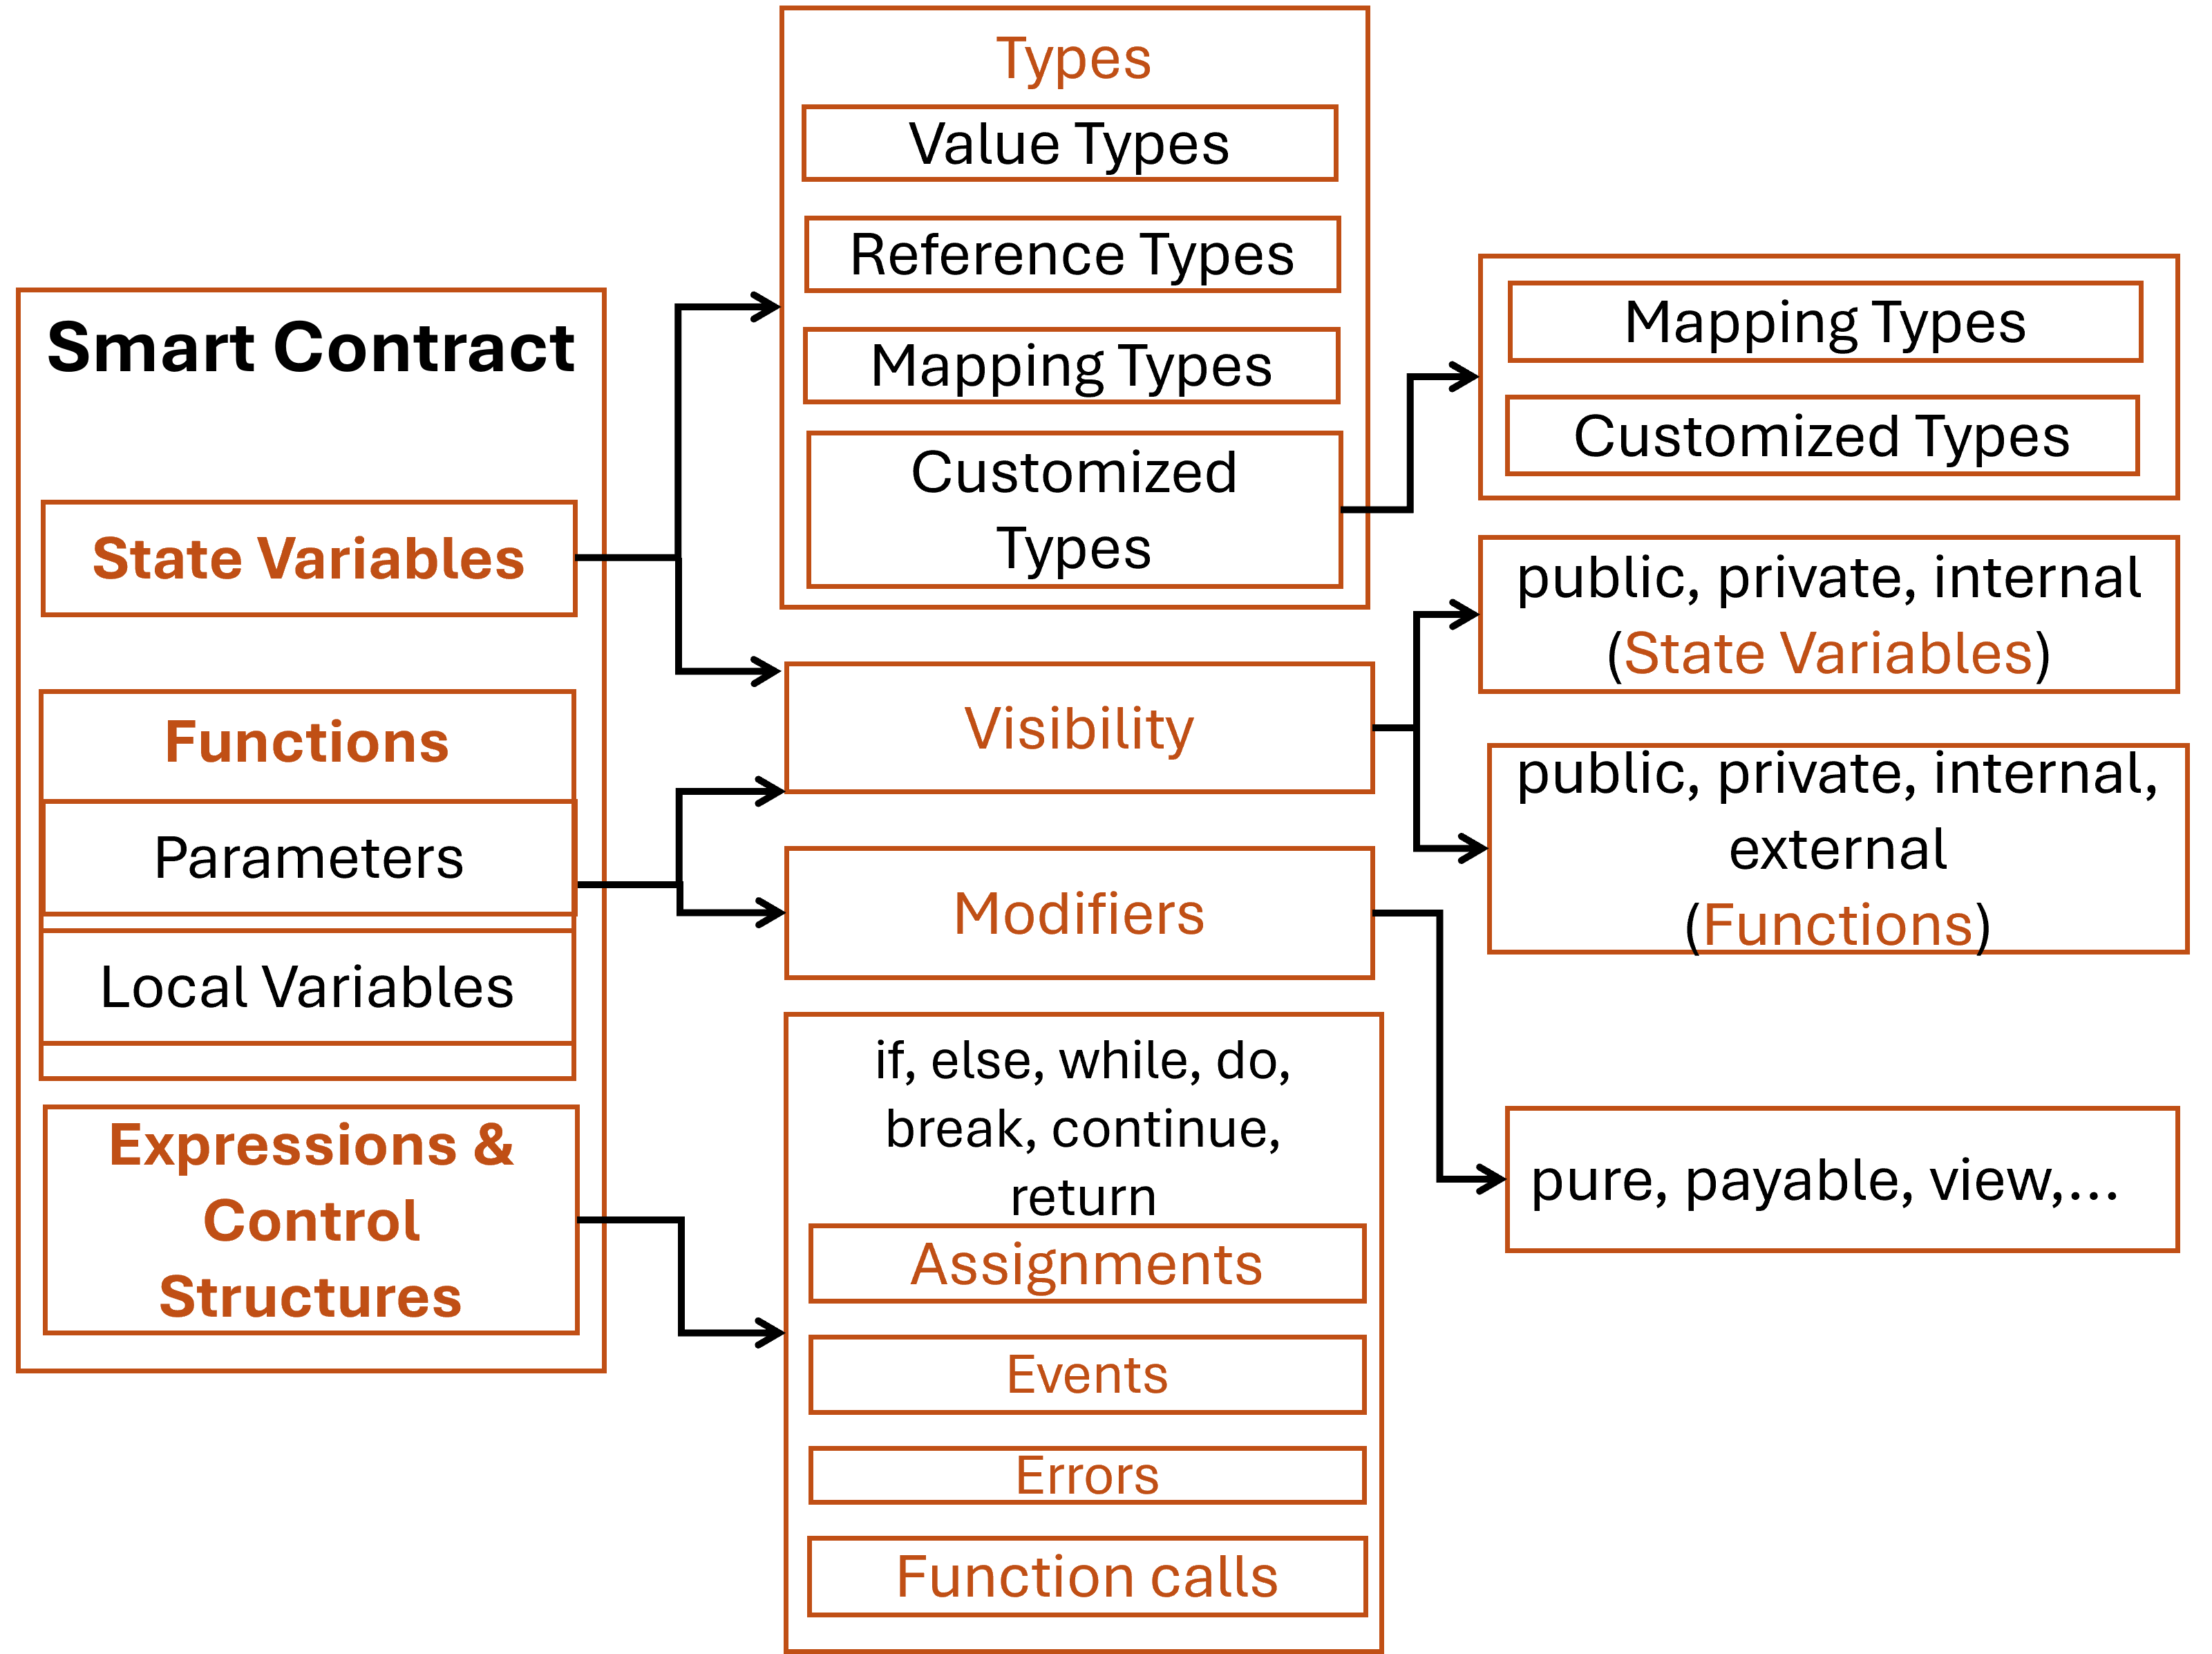
\includegraphics[width=10cm,keepaspectratio]{solidityl.PNG}
%	\end{center}
%\end{frame}

%
\subsection{Proposed Methodology}
\begin{frame}{Proposed Methodology}
\begin{figure}[!h]
\centering
%\begin{tikzpicture}[show background grid]
\begin{tikzpicture}[]
%PICTURE SCOPE or REFERENCEs
\node at (0, 0) (topleft) [circle] {};
%\node at (11.75, 0) (topright) [circle, draw=red, fill=red] {};
\node (topright) [circle, xshift = 10.5cm, right of = topleft] {};
\node (bottomleft) [circle, yshift = -7.25cm, below of = topleft] {};
\node (bottomright) [circle, xshift = 11.5cm, yshift = -7.25cm, below of = topleft] {};
%\draw (0,-3) [draw=red, fill=red]  -- (5, -4); % CHECK once of the grid is affecting the placement of the objects
%GRID

 \draw (2, -0.45 ) [rounded corners = 4pt, draw=black, fill=blue!4]  -- ++(8.15cm, 0) node[below left] {\textcolor{blue}{\scriptsize{Isabelle/Soildity}}}  --++(0, -5.5cm) --++(-8.15, 0)--cycle;
\draw (2, -0.35 ) [rounded corners = 4pt, draw=black, fill=red!4]  -- ++(8.18cm, 0)  --++(0, 1.3cm) --++(-8.15, 0)node[below right, xshift=2.8cm] {\textcolor{red}{\scriptsize Solidity (v 0.8.25)}}-- cycle;
%\draw (2.5, -0.65) [rounded corners = 4pt, draw=black, fill=blue!4]  -- ++(5cm, 0) --++(0, -2.65cm)--++(-5, 0)--cycle;
%\draw (2.65, -0.85) [rounded corners = 4pt, draw=black, fill=blue!4]  -- ++(3.1cm, 0) --++(0, -2.3cm)--++(-3.1, 0)--cycle;
%INPUTS
%\node (solidity) [thin, draw=black, fill=red!4,  rectangle, rounded corners= 2pt, xshift = 4.40cm, right of = topleft, inner sep = 4pt] {\scriptsize Solidity (v 0.8.25)};
\node (model) [thin, draw=black, fill=red!4,  minimum height= 0.6cm, rectangle, rounded corners= 2pt, xshift = 1.65cm, yshift = 0.10cm, right of = topleft, inner sep = 4pt] {\scriptsize Model};
\node (spec) [thin, draw=black, fill=red!4,  minimum height= 0.6cm, rectangle, rounded corners= 2pt, xshift = 3.40cm, yshift = 0.10cm, right of = topleft, inner sep = 4pt] {\scriptsize Specifications};
\node (ver) [thin, draw=black, fill=red!4,  minimum height= 0.6cm, rectangle, rounded corners= 2pt, xshift = 6.850cm, yshift = 0.10cm, right of = topleft, inner sep = 4pt] {\scriptsize{ Verification Condition Generator}};
\onslide<2->\node (sm) [thin, draw=black, fill=blue!4,  rectangle, minimum width=2.3cm, rounded corners= 2pt, xshift = 2.85cm, yshift = -1.25cm, right of = topleft, inner sep = 4pt, align = center] {\scriptsize Isabelle/HOL};
\node (sm1) [thin, draw=black, fill=blue!4,  rectangle, minimum width=2.3cm,  xshift = 2.85cm, yshift = -2.10cm, right of = topleft, inner sep = 2pt, align = center] {\scriptsize{ State.thy,} \\[0.15] \scriptsize{State\_monad.thy,} \\[0.15] \scriptsize{Solidity.thy}};
%
%MODEL TO SM
%\draw  [draw=black, line width = 1.5pt, ->] (model.south)  to [out=270, in=90] (sm.north);; ;;
\draw  [draw=black, line width = 1.5pt, ->] (model.south)  --++(0, -0.35cm) |- (3.25cm, -0.65cm) -| (sm.north);; ;;
%%SM TO HOL CORE
\draw  [draw=black, line width = 1.5pt, <->] (sm.east)  -- ++(3.35cm, 0);;;; ;;
%
\node (dtl) [thin, draw=black, fill=blue!4,  rectangle, minimum width=4.9cm, rounded corners= 2pt, xshift = 7.90cm, yshift = -3.35cm, right of = topleft, inner sep = 4pt, align = center, rotate=90] { {\scriptsize \textcolor{white}{Isabelle/HOL}}\\[0.15] {\scriptsize \textcolor{white}{ Definitions/Thoerems/Lemmas}}};
\node (dtl) [thin, draw=black, fill=blue!4,  rectangle, minimum width=4.9cm, rounded corners= 2pt, xshift = 8cm, yshift = -3.45cm, right of = topleft, inner sep = 4pt, align = center, rotate=90] { {\scriptsize Isabelle/HOL}\\[0.15] {\scriptsize  Definitions/Thoerems/Lemmas}};
\node (isac) [thin, draw=black, fill=blue!4,  rectangle, rounded corners= 2pt, minimum width= 5.5cm, xshift = 9.75cm,  yshift= -3.2cm, right of = topleft,  inner sep = 4pt,   align = center, rotate=90] { {\scriptsize Isabelle/HOL Core}};
\draw  [draw=black, line width = 1.5pt, <->] (9.52, -3) -- ++(0.95cm, 0) ;;
%%THEORIES-step02

\onslide<3->\node (isasol) [thin, draw=black, fill=blue!4,  rectangle, minimum width=2.3cm, rounded corners= 2pt, xshift = 4.550cm, yshift = -3.55cm, right of = topleft, inner sep = 4pt, align = center] {\scriptsize Isabelle/ML};
\node (isasol1) [thin, draw=black, fill=blue!4,  rectangle, minimum width=2.3cm,  xshift = 4.550cm, yshift = -4.05cm, right of = topleft, inner sep = 4pt, align = center] {\scriptsize{ Contract.thy}};
%SPECIFICATION TO CONTRACT
\draw  [draw=black, line width = 1.5pt, ->] (spec.south)  --++(0, -0.35cm) |- (5.25cm, -0.65cm) -| (isasol.north);; ;;
%%Contract to Modeling
\draw  [draw=black, line width = 1.5pt, <->]  (sm1.south east) --++ (0, -0.5);;
\draw  [draw=black, line width = 1.5pt, ->] (isasol.east) -- ++(1.65cm, 0);;
%
%
%
\onslide<4->\node (sc) [thin, draw=black, fill=red!4,  rectangle, rounded corners= 2pt, xshift= -0.75cm, yshift = -3.55cm, right of = topleft, inner sep = 4pt, align = center] {\scriptsize Smart Contract  \&\\[0.05pt] \scriptsize Property Specification };
\draw  [draw=black, line width = 1.5pt, ->] (sc.east) to [ out=360, in=180] (isasol.west);;
\node (vsc) [thin, draw=black, fill=green!10,  rectangle, rounded corners= 2pt, minimum width= 5.5cm, xshift = 10.75cm,  yshift= -3.2cm, right of = topleft,  inner sep = 4pt,   align = center, rotate=90] { {\scriptsize Verified Smart Contract}};
\draw  [draw=black, line width = 1.5pt, ->] (11.01, -3) -- ++(0.5cm, 0) ;;
\onslide<5->\node (vcg) [thin, draw=black, fill=blue!4,  rectangle, minimum width=2.3cm, rounded corners= 2pt, xshift = 5.90cm, yshift = -5.10cm, right of = topleft, inner sep = 4pt, align = center] {\scriptsize \scriptsize Isabelle/HOL};

\node (vcg1) [thin, draw=black, fill=blue!4,  rectangle, minimum width=2.3cm, xshift = 5.90cm, yshift = -5.60cm, right of = topleft, inner sep = 4pt, align = center] {\scriptsize{ WP.thy}};


%%CONNECTIONS
%

\node (scp) [thin, draw=black, fill=red!4,  rectangle, rounded corners= 2pt, xshift = -0.80cm, yshift = -5.50cm, right of = topleft, inner sep = 4pt, align = center] {\scriptsize Automatic  Verification};
%
%scp to verification generator
\draw  [draw=black, line width = 1.5pt, <-]  (vcg1.west) --++ (-4.0cm, 0);;
%vcg to modeling
\draw  [draw=black, line width = 1.5pt, <->]  (vcg.west) --++(-1.8cm, 0) -| (sm1.south);;
%Contract to verification generator
\draw  [draw=black, line width = 1.5pt, <->]  (vcg.north west) --++ (0, 0.5);;
%
%%INTERCONECTIONS
%\draw  [draw=black, line width = 1.5pt, ->] (solidity.south) --  ++(0, -0.60cm) ;;
%\draw  [draw=black, line width = 1.5pt, <->] (sm1.south)  to [out=270, in=90] (isasol.north);; ;;
%\draw  [draw=black, line width = 1.5pt, <->] (isasol1.south)  to [out=270, in=90] ++(0, -1.10);; ;;
%%SM1 TO DTL
%\draw  [draw=black, line width = 1.5pt, ->] (5.75, -2.35) -- ++(2.72cm, 0) ;;
%\draw  [draw=black, line width = 1.5pt, -] (5.75, -2) -- ++(0, -0.38cm) ;;



%DTL TO CORE
%
%%
%
%%
%\draw  [draw=black, line width = 1.5pt, ->] (vcg.north west) to [out=90, in=-90]   ++(0, 0.38cm)|- (sm.west) ;;


%WP to VCG
\draw  [draw=black, line width = 1.5pt, <-] (vcg.north)  --++(0, 4.63cm) ;; ;;

\end{tikzpicture}

\end{figure}
\end{frame}

%\subsection{Solidity}
%\begin{frame}{Solidity Smart Contract}
%	\begin{center}
%	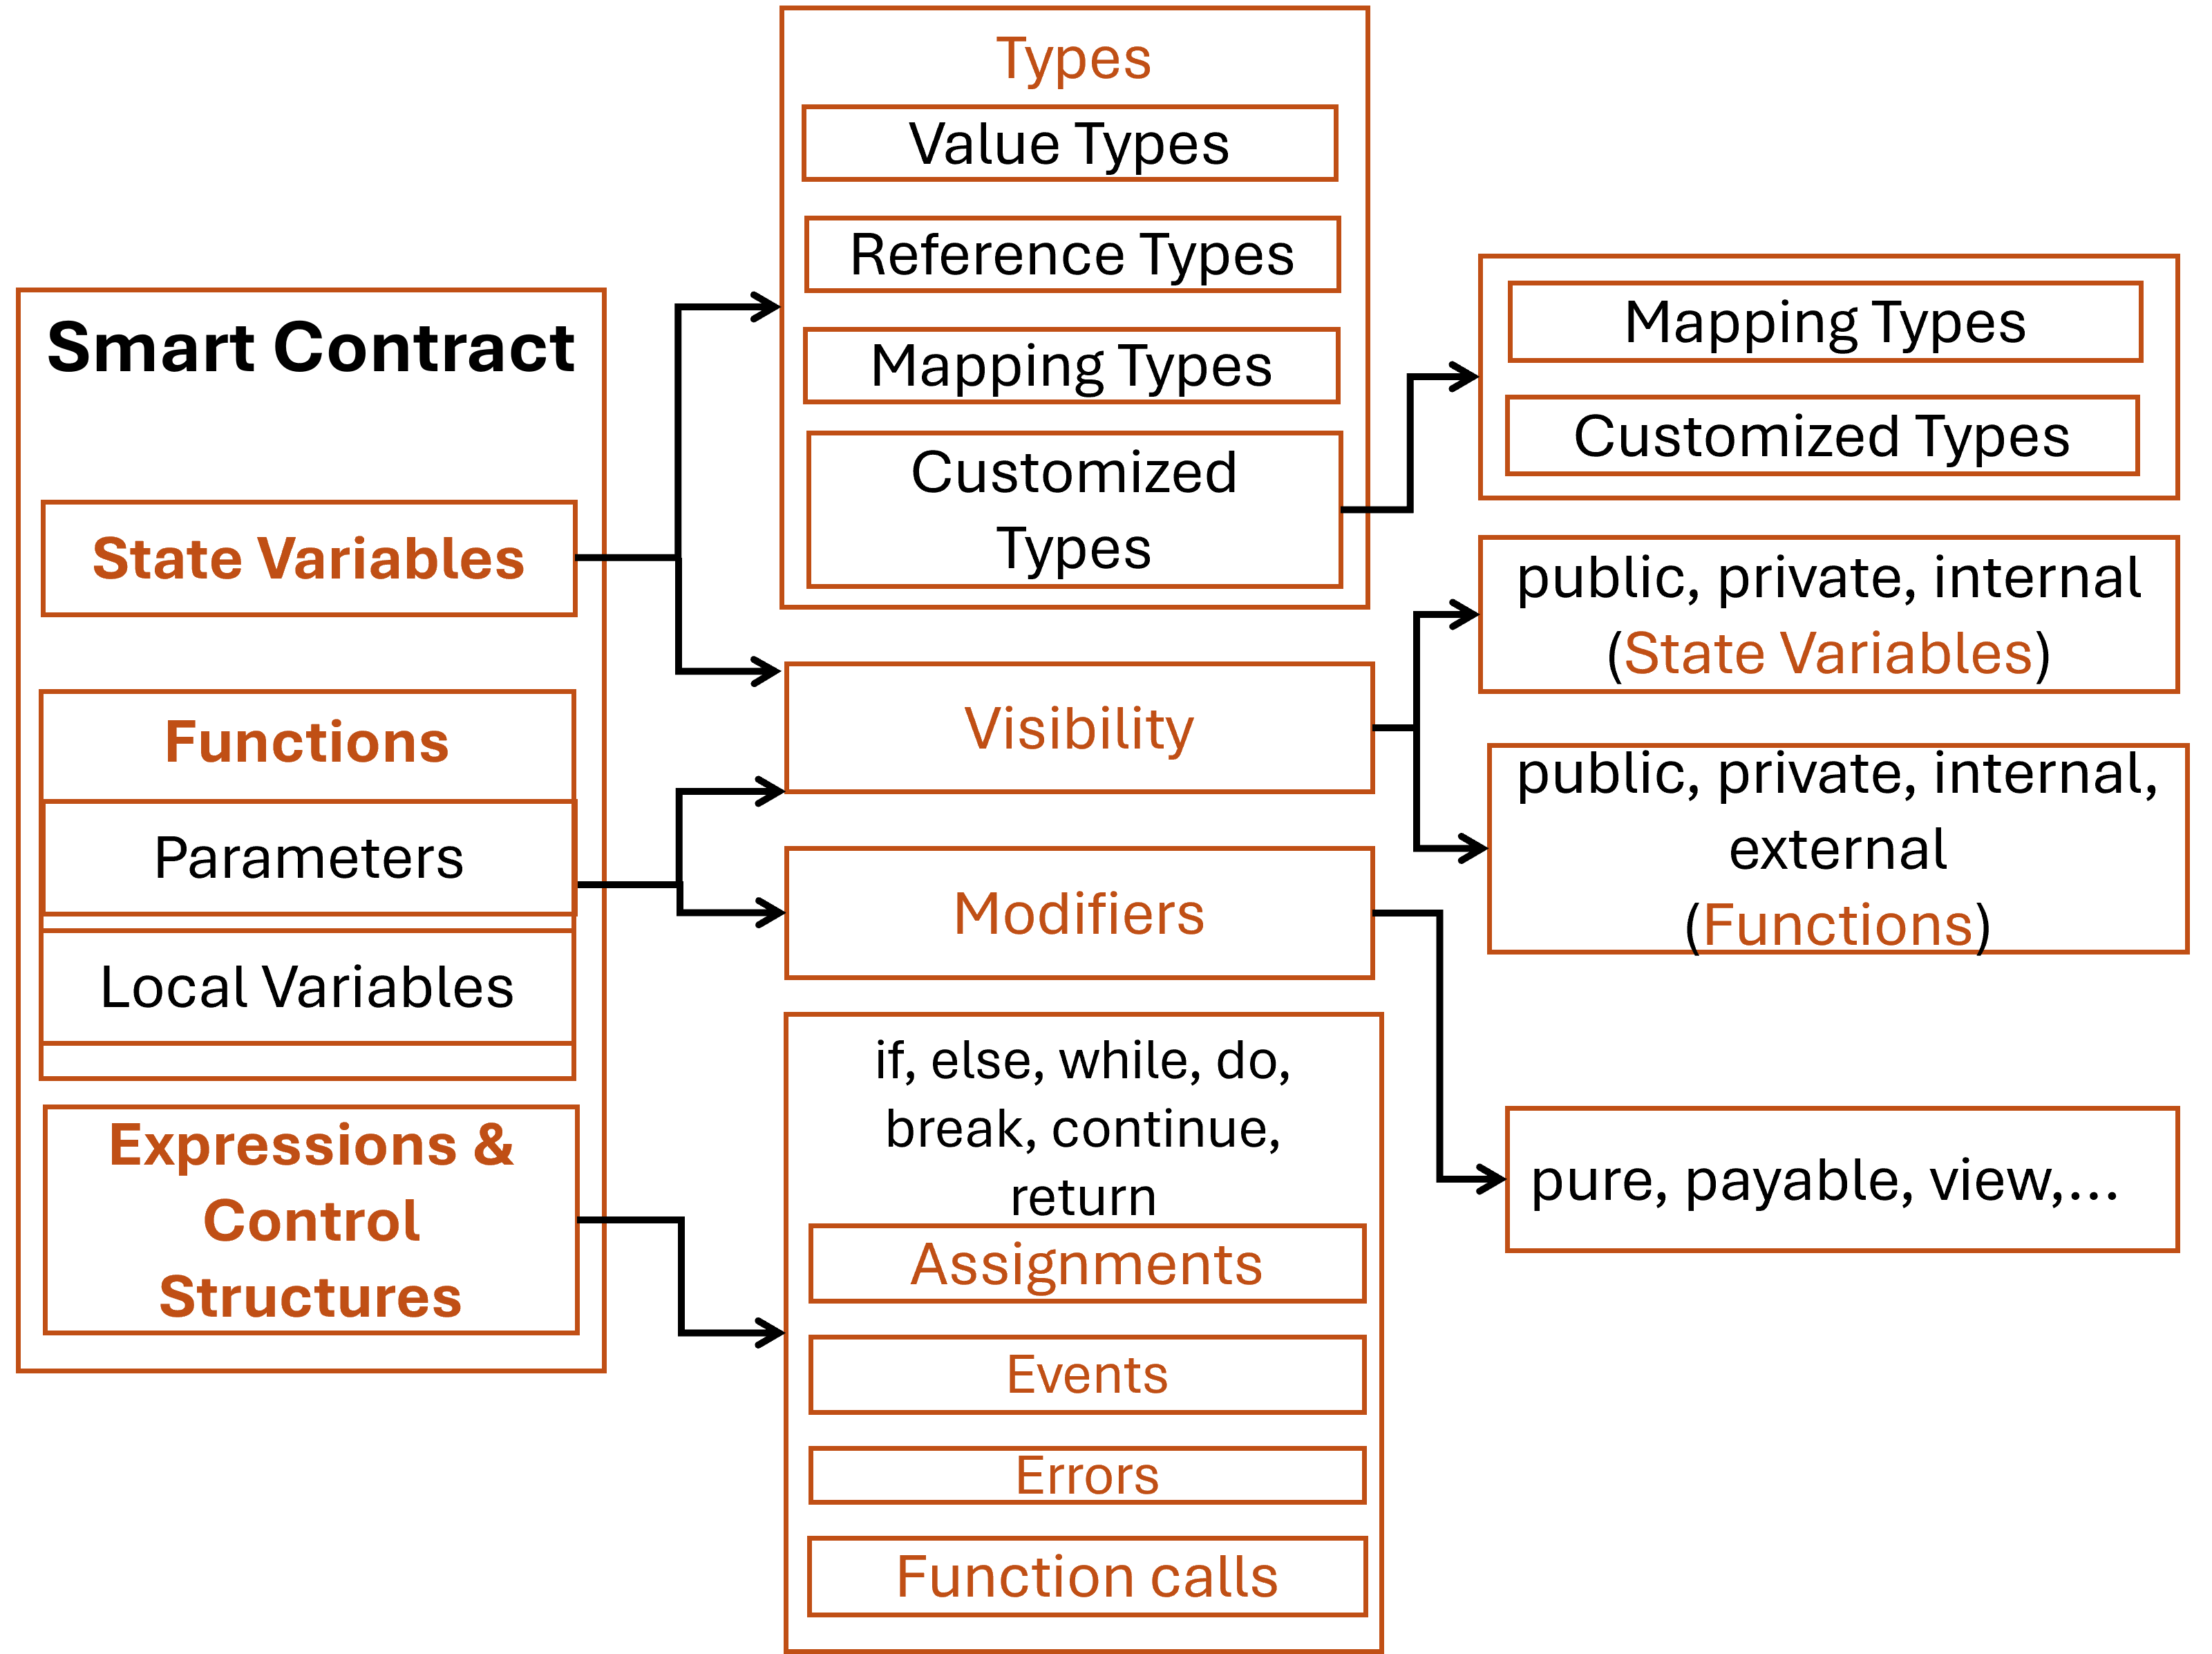
\includegraphics[width=10cm,keepaspectratio]{solidityl.PNG}
%	\end{center}
%\end{frame}
%
%\begin{frame}{Solidity Store Types}
%	\begin{center}
%	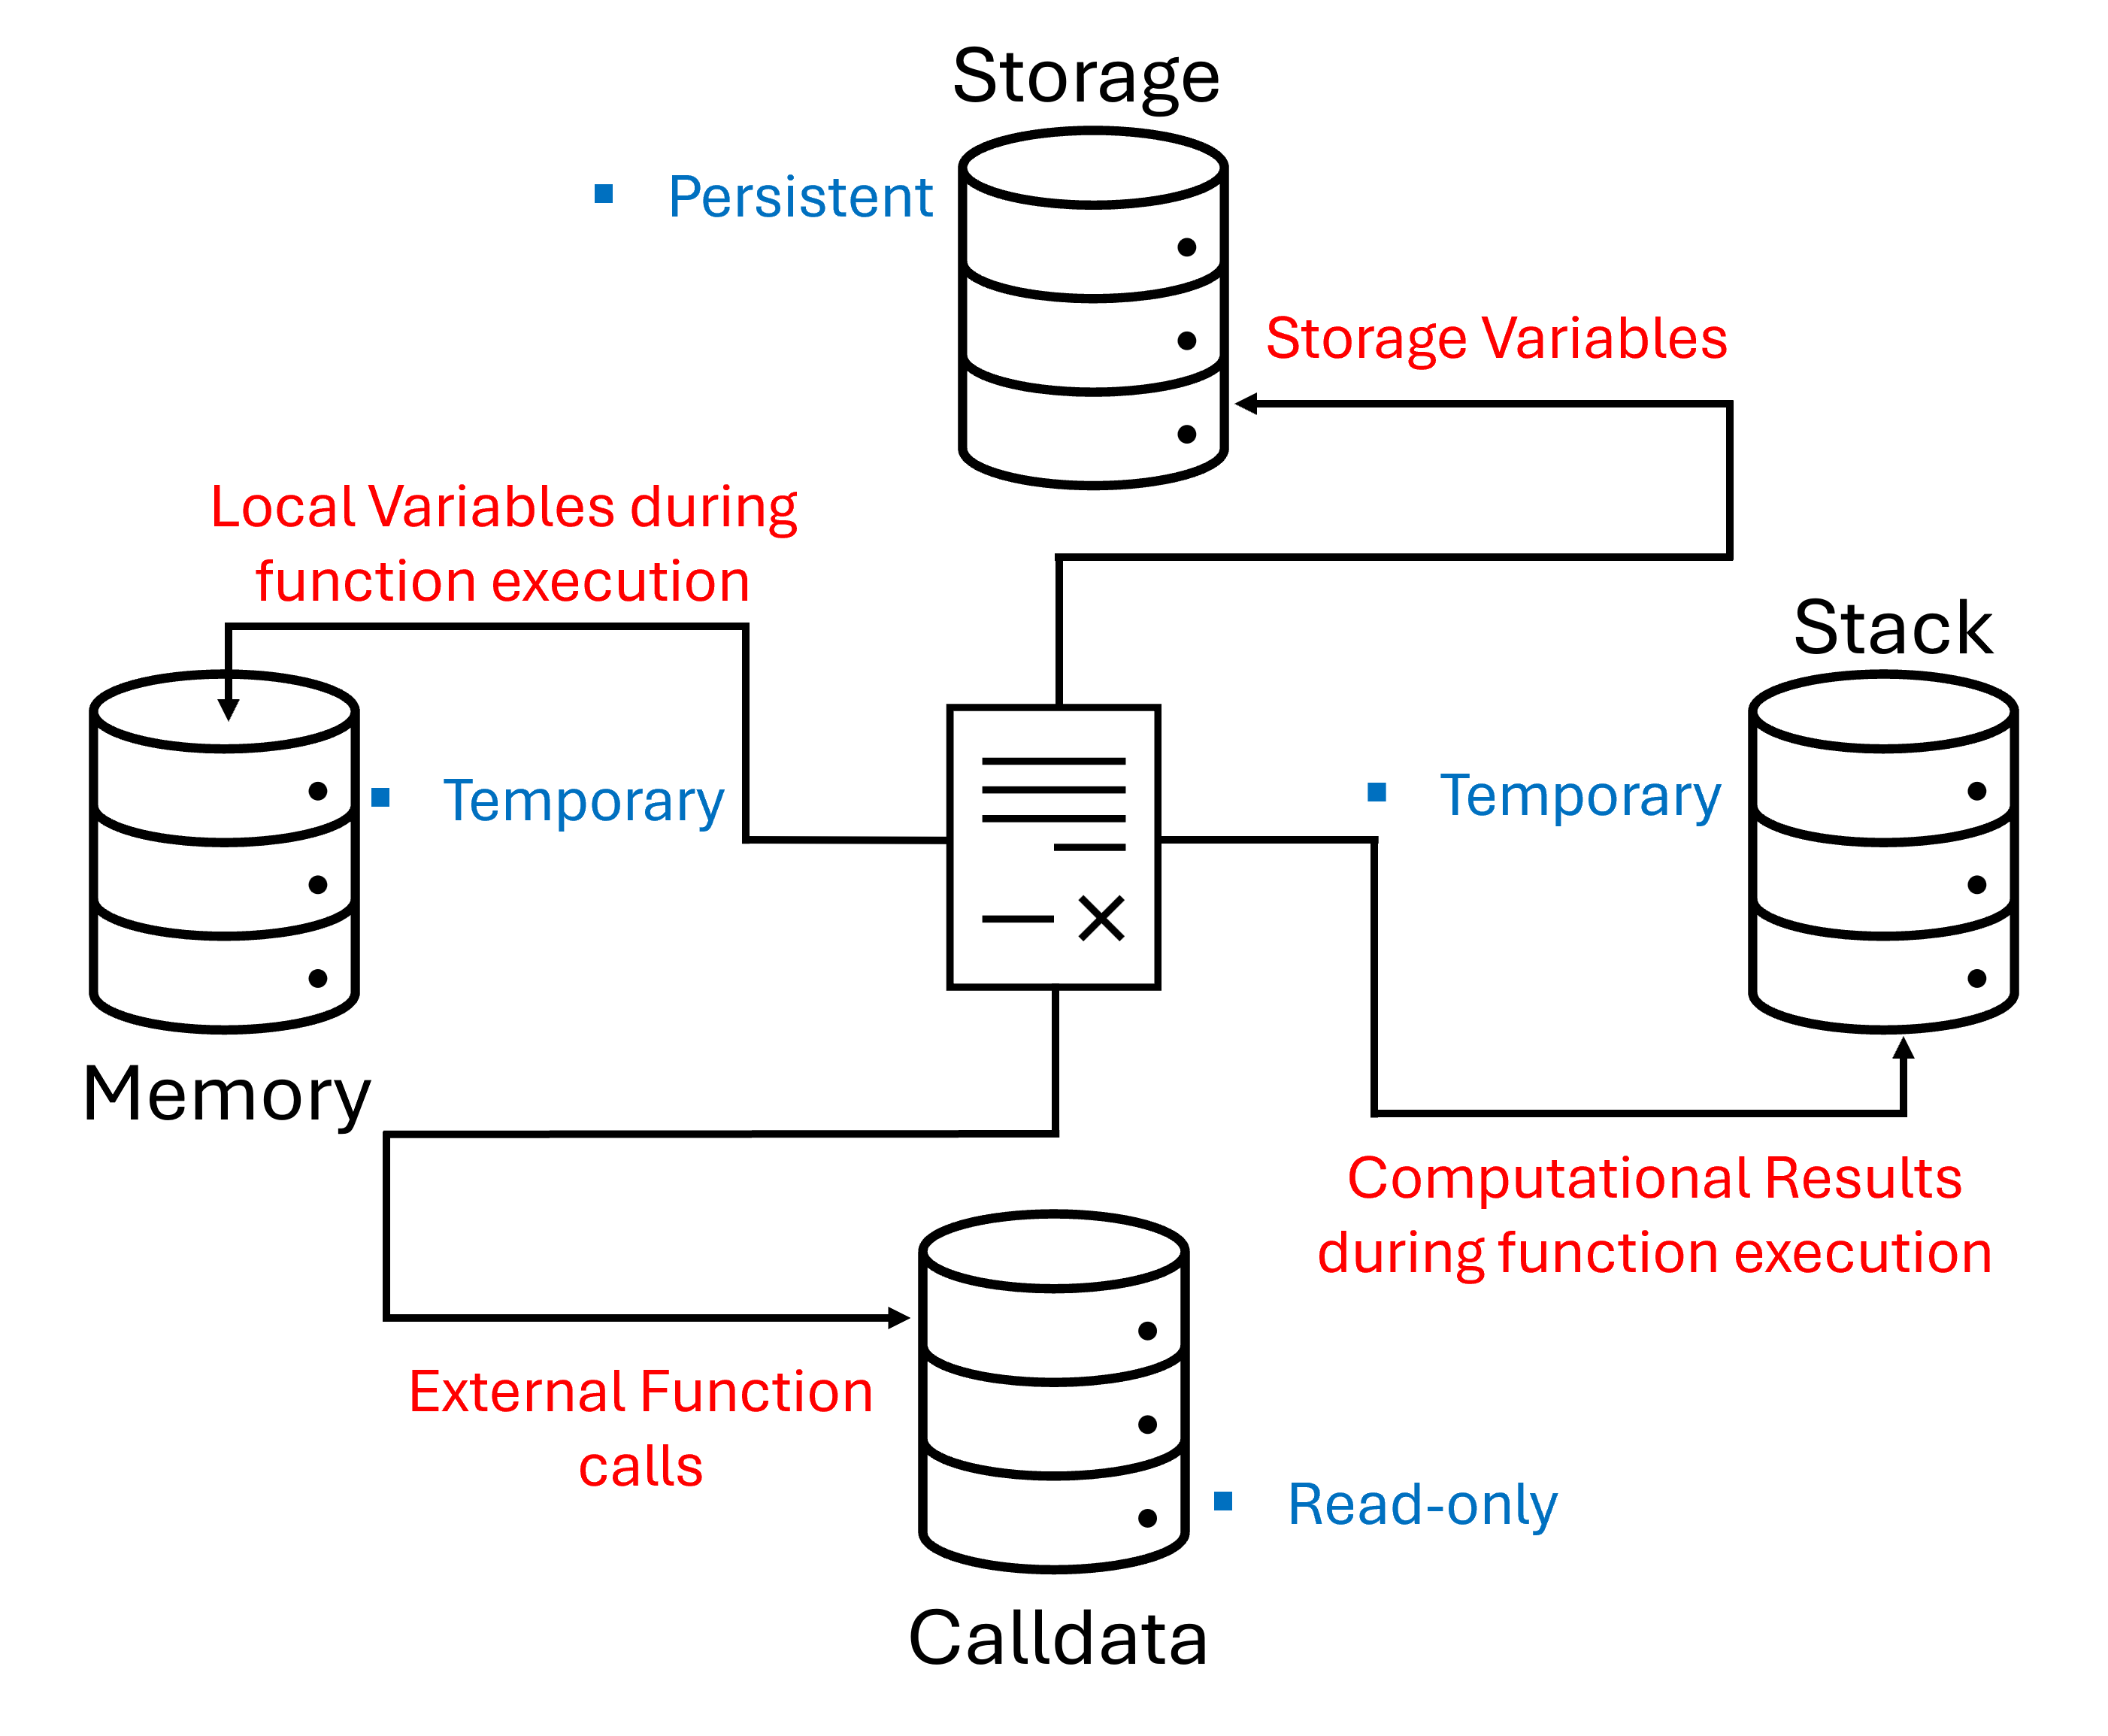
\includegraphics[width=7.5cm,keepaspectratio]{datatypes.PNG}
%	\end{center}
%\begin{exampleblock}{}
%  {\large \begin{center}Store types are critical to the syntax and semantics of Solidity\end{center}}
%\end{exampleblock}
%\end{frame}


\section{Solidity}
\frame{\tableofcontents[currentsection]}

%\begin{frame}{Bank}
%\begin{itemize}
%\item Keeps an internal record of funds transferred by its customers.
%\item This record is increased whenever a customer transfers additional funds 
%\item When customer withdraws all its recorded
%funds are returned and its internal record reset to 0.
%\end{itemize}
\subsection{Example Contract}
%
\begin{frame}{Banking Smart Contract}
\begin{tikzpicture}
    \node[anchor=south west,inner sep=0] (image) at (0,0) {
 \begin{minipage}[t]{0.90\textwidth}
\begin{soliditybox}
pragma solidity >=0.5.1 <0.5.2;

contract Bank {
    mapping(address => uint256) balances;

    function deposit() public payable {
        balances[msg.sender] = balances[msg.sender] + msg.value;
    }

    function withdraw() public {
        uint256 bal = balances[msg.sender];
        balance[msg.sender] = 0;
        msg.sender.transfer(bal);
    }
}
\end{soliditybox}
\end{minipage}};
\pause\begin{scope}[x={(image.south east)},y={(image.north west)}]
      \draw[red,ultra thick,rounded corners] (0.13,0.05) rectangle (0.9,0.15) ;
	\node at (0.5, 0.1) (inv) [] {\textcolor{red}{Invariant:} balance of contract $\leq$ Sum of deposits};
    \end{scope}
\end{tikzpicture}
\end{frame}
%%
%%
\section{Isabelle/Solidity}
\subsection{Specification}
\begin{frame}{Specification}

\begin{Example}{}{}
	The formalization of our example :
	\begin{center}
		\fbox{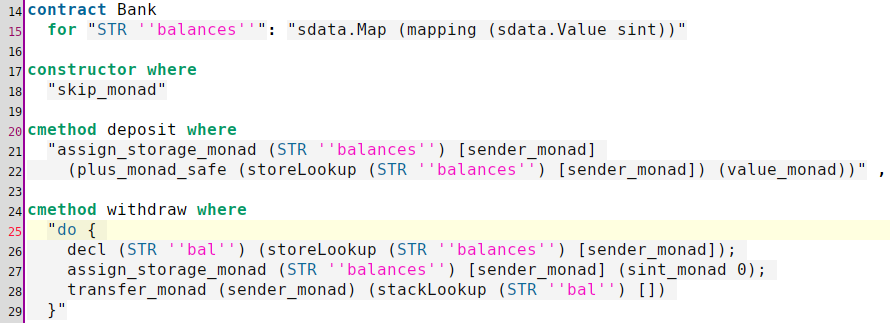
\includegraphics[width = 11.5cm]{bank_spec.png}}
	\end{center}
\end{Example}
\end{frame}
%%
%%
%%
\subsection{Verification}
\begin{frame}{Invariance Verification}
\begin{Example}{}{}
\begin{align*}
		\mathit{Invariance}\colon&\mathit{\color{blue}balance} \geq \sum_{\{(a,x)|\texttt{balances}(a)=x\}} x\\
	\end{align*}
		\begin{center}\vspace{-2mm}
		\fbox{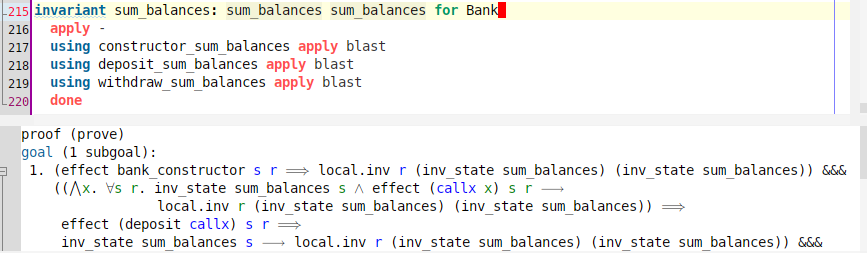
\includegraphics[width=.95\textwidth]{invariant.png}}
	\end{center}\vspace{-2mm}
Output window shows proof obligations discharged using lemmas.
\end{Example}
\end{frame}
%
%%%%
\begin{frame}{Verification Condition Generator (VCG)}
\begin{Example}{}{}
	Using VCG to automatically discharge proof obligations for deposit method.\\
		\fbox{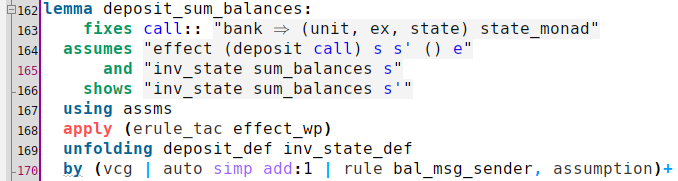
\includegraphics[width=.95\textwidth]{deposit.png}}
	\end{Example}
\end{frame}
%
\begin{frame}{Case Studies}
\begin{columns}
\column{.48\textwidth}
\begin{itemize}
\item \textcolor{red}{Specification} (\textbf{black}) and \textcolor{red}{verification} (\textbf{grey}) effort in terms of lines of proof code
\item \textcolor{red}{Casino} from “VerifyThis long-term verification
challenge”
\item \textcolor{red}{Voting} from Solidity official documentation
\item Verifying invariant for \textbf{Bank} with Approx. \textcolor{red}{100 lines of code}, a reduction by \textcolor{red}{ 97\%} compared to Deep embedding 


\end{itemize}

\column{.48\textwidth}
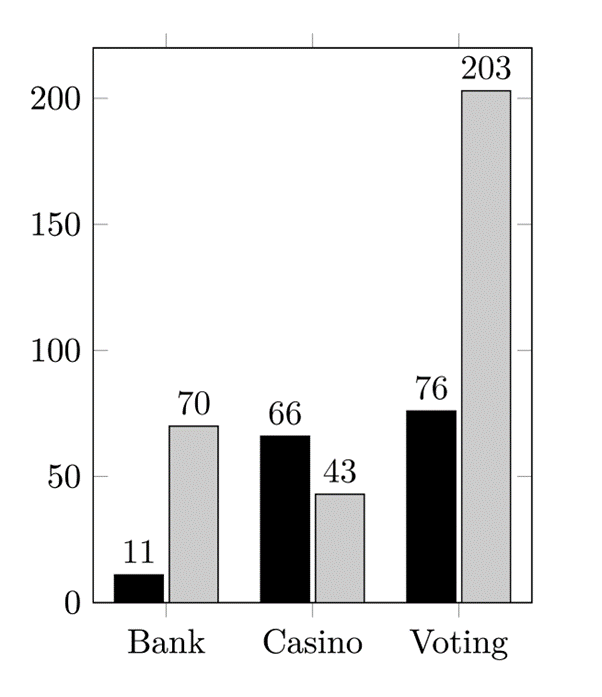
\includegraphics[width=\columnwidth, height=6cm,
  keepaspectratio]{graph.png}
\end{columns}
\end{frame}
%
\section{Conclusion}
\frame{\tableofcontents[currentsection]}

\begin{frame}{Conclusion}
Summary
\begin{itemize}
	\item \textcolor{red}{Shallow embedding} of subset of Solidity in Isabelle/HOL
	\item Test suit for  \textcolor{red}{semantics conformance testing}
	\item A \textcolor{red}{verification condition generator} for \textcolor{red}{automation}
	\item Used to verify \textcolor{red}{concrete Solidity contracts} from \textcolor{red}{official documentation of Solidity}
%	\item Proposed methodology reduced effort for verifying invariant with \textcolor{red}{100 lines of code}, a reduction by \textcolor{red}{ 97\%} compared to Deep embedding 
\end{itemize}
\bigskip

Limitations: 
\begin{itemize}
	\item Some advanced features are still missing: \textcolor{red}{inheritance}, \textcolor{red}{visibility}, \textcolor{red}{modifiers}
\end{itemize}
\end{frame}
%%%%%%%%%%%
\begin{frame}{}
	\begin{center}
{\fontsize{40}{50}\selectfont Thank You!}\\
\vspace{0.5in}
{\fontsize{30}{40}\selectfont \textcolor{white}{\colorbox{blue}{Q\&A}}}\\
\end{center}
\end{frame}
%%%%%%%%%
%
%\begin{frame}{Future Work}
%\begin{figure}[!h]
%\centering
%%\begin{tikzpicture}[show background grid]
%\begin{tikzpicture}[]
%%PICTURE SCOPE or REFERENCEs
%\node at (0, 0) (topleft) [circle] {};
%%\node at (11.75, 0) (topright) [circle, draw=red, fill=red] {};
%\node (topright) [circle, xshift = 10.5cm, right of = topleft] {};
%\node (bottomleft) [circle, yshift = -7.25cm, below of = topleft] {};
%\node (bottomright) [circle, xshift = 11.5cm, yshift = -7.25cm, below of = topleft] {};
%%\draw (0,-3) [draw=red, fill=red]  -- (5, -4); % CHECK once of the grid is affecting the placement of the objects
%%GRID
%%\node (0.5, -2.5)(para) [thin, draw=black, fill=red!4,  minimum height= 0.6cm, rectangle, rounded corners= 2pt, inner sep = 4pt] {\scriptsize Parameters};
%\draw (-0.25, -0.75 ) [rounded corners = 4pt, draw=black, fill=green!10]  -- ++(2.6cm, 0) node[below left, xshift=-0.15cm] {\textcolor{blue}{\scriptsize{Smart Contracts}}}  --++(0, -5.0cm) --++(-2.6, 0)--cycle;
%\node (para) [thin, draw=black,  minimum width=2.15cm, rectangle, rounded corners= 2pt, yshift = -3cm, right of = topleft, inner sep = 4pt, align = center] { \scriptsize Parameters};
%\node (lv) [thin, draw=black,  minimum width=2.15cm, rectangle, rounded corners= 2pt, yshift = -3.75cm, right of = topleft, inner sep = 4pt, align = center] { \scriptsize Local Variables};
%
% \node (fun) [
%          fit=(para) (lv),
%          yshift=0.2cm, inner ysep=0.4cm,inner xsep=0.05cm,
%          draw, 
%         label={[label distance=-0.50cm]north:\scriptsize{Functions}}, rounded corners] {};
%\node (ecs) [thin, draw=black,  minimum width=2.230cm, rectangle, rounded corners= 2pt, yshift = -5cm, right of = topleft, inner sep = 4pt, align = center] { \scriptsize{Expressions \&}\\[-1.5pt]\scriptsize{Control}\\[-1.5pt]\scriptsize{Structures}};
%\node (sv) [thin, draw=black,  minimum width=2.230cm, rectangle, rounded corners= 2pt, yshift = -01.75cm, right of = topleft, inner sep = 4pt, align = center] { \scriptsize State Variables};
%%%%%%%3rd COlumn
%\node (mt) [thin, draw=black,  minimum width=2.55cm, rectangle, rounded corners= 2pt, xshift=9cm,  yshift = -0.80cm, right of = topleft, inner sep = 4pt, align = center] { \scriptsize Mapping Types};
%\node (ct) [thin, draw=black,  minimum width=2.55cm, rectangle, rounded corners= 2pt, xshift=9cm,  yshift = -01.55cm, right of = topleft, inner sep = 4pt, align = center] { \scriptsize Customized Types};
% \node (mtct) [
%          fit=(mt) (ct),  draw,  thin] {};
%%%
%\node (vis1) [thin, draw=black,  minimum width=2.55cm, rectangle, rounded corners= 2pt, xshift=9cm,  yshift = -2.80cm, right of = topleft, inner sep = 4pt, align = center] { \scriptsize{ private, public}\\[-1pt] \scriptsize{ internal}\\[-1pt]  \scriptsize{ \textcolor{red}{(State Variables)}}};
%\node (vis2) [thin, draw=black,  minimum width=2.55cm, rectangle, rounded corners= 2pt, xshift=9cm,  yshift = -4.35cm, right of = topleft, inner sep = 4pt, align = center] { \scriptsize{ private, public}\\[-1pt] \scriptsize{ internal, external}\\[-1pt]  \scriptsize{ \textcolor{red}{(Functions)}}};
%%
%\node (mod1) [thin, draw=black,  minimum width=2.55cm, rectangle, rounded corners= 2pt, xshift=9cm,  yshift = -5.65cm, right of = topleft, inner sep = 4pt, align = center] { \scriptsize{ pure, payable}\\[-1pt] \scriptsize{ veiw...}};
%\end{tikzpicture}
%\end{figure}
%\end{frame}

%
%\begin{frame}{Project Proposal}
%	Aim: A verified tool which takes as input an annotated Solidity contract and generates a verification condition which can be discharged in Isabelle/HOL
%	\bigskip\pause
%
%	Objectives
%	\begin{itemize}
%		\item Develop a calculus to reason about semantics and implement it in Isabelle
%		\item Implement a Verification Condition Generator
%		\item Organize a smart contract verification competition
%	\end{itemize}
%	\bigskip\pause
%
%	Team
%	\begin{itemize}
%		\item Myself: Work on semantics
%		\item Prof. Achim Brucker: Expert in Isabelle
%		\item Postdoc (to be funded by the grant)
%		\item PhD student (funded by University of Exeter)
%	\end{itemize}
%\end{frame}
%
%\begin{frame}{Possibilities for Collaboration}
%	Required: A supporting statemement for the proposal
%	\begin{itemize}
%		\item Confirmation that the project is interesting
%		\item Usually some (unbinding) commitment for some type of support\\
%		(usually in terms of time spent on the project)
%	\end{itemize}
%	\bigskip\pause
%
%	Desired: Ongoing discussions, feedback, ideas
%	\begin{itemize}
%		\item Regular meetings to discuss progress
%		\item Insights into practical examples
%		\item Feedback about usability
%		\item Ideas for improvements
%		\item Collaboration on publications
%	\end{itemize}
%\end{frame}
%
%\begin{frame}[allowframebreaks]{References}
%	\nocite{*}
%	\bibliographystyle{unsrt}
%	\bibliography{references.bib}
%\end{frame}

\end{document}